\documentclass[twoside]{book}

% Packages required by doxygen
\usepackage{fixltx2e}
\usepackage{calc}
\usepackage{doxygen}
\usepackage[export]{adjustbox} % also loads graphicx
\usepackage{graphicx}
\usepackage[utf8]{inputenc}
\usepackage{makeidx}
\usepackage{multicol}
\usepackage{multirow}
\PassOptionsToPackage{warn}{textcomp}
\usepackage{textcomp}
\usepackage[nointegrals]{wasysym}
\usepackage[table]{xcolor}

% Font selection
\usepackage[T1]{fontenc}
\usepackage[scaled=.90]{helvet}
\usepackage{courier}
\usepackage{amssymb}
\usepackage{sectsty}
\renewcommand{\familydefault}{\sfdefault}
\allsectionsfont{%
  \fontseries{bc}\selectfont%
  \color{darkgray}%
}
\renewcommand{\DoxyLabelFont}{%
  \fontseries{bc}\selectfont%
  \color{darkgray}%
}
\newcommand{\+}{\discretionary{\mbox{\scriptsize$\hookleftarrow$}}{}{}}

% Page & text layout
\usepackage{geometry}
\geometry{%
  a4paper,%
  top=2.5cm,%
  bottom=2.5cm,%
  left=2.5cm,%
  right=2.5cm%
}
\tolerance=750
\hfuzz=15pt
\hbadness=750
\setlength{\emergencystretch}{15pt}
\setlength{\parindent}{0cm}
\setlength{\parskip}{3ex plus 2ex minus 2ex}
\makeatletter
\renewcommand{\paragraph}{%
  \@startsection{paragraph}{4}{0ex}{-1.0ex}{1.0ex}{%
    \normalfont\normalsize\bfseries\SS@parafont%
  }%
}
\renewcommand{\subparagraph}{%
  \@startsection{subparagraph}{5}{0ex}{-1.0ex}{1.0ex}{%
    \normalfont\normalsize\bfseries\SS@subparafont%
  }%
}
\makeatother

% Headers & footers
\usepackage{fancyhdr}
\pagestyle{fancyplain}
\fancyhead[LE]{\fancyplain{}{\bfseries\thepage}}
\fancyhead[CE]{\fancyplain{}{}}
\fancyhead[RE]{\fancyplain{}{\bfseries\leftmark}}
\fancyhead[LO]{\fancyplain{}{\bfseries\rightmark}}
\fancyhead[CO]{\fancyplain{}{}}
\fancyhead[RO]{\fancyplain{}{\bfseries\thepage}}
\fancyfoot[LE]{\fancyplain{}{}}
\fancyfoot[CE]{\fancyplain{}{}}
\fancyfoot[RE]{\fancyplain{}{\bfseries\scriptsize Generated by Doxygen }}
\fancyfoot[LO]{\fancyplain{}{\bfseries\scriptsize Generated by Doxygen }}
\fancyfoot[CO]{\fancyplain{}{}}
\fancyfoot[RO]{\fancyplain{}{}}
\renewcommand{\footrulewidth}{0.4pt}
\renewcommand{\chaptermark}[1]{%
  \markboth{#1}{}%
}
\renewcommand{\sectionmark}[1]{%
  \markright{\thesection\ #1}%
}

% Indices & bibliography
\usepackage{natbib}
\usepackage[titles]{tocloft}
\setcounter{tocdepth}{3}
\setcounter{secnumdepth}{5}
\makeindex

% Hyperlinks (required, but should be loaded last)
\usepackage{ifpdf}
\ifpdf
  \usepackage[pdftex,pagebackref=true]{hyperref}
\else
  \usepackage[ps2pdf,pagebackref=true]{hyperref}
\fi
\hypersetup{%
  colorlinks=true,%
  linkcolor=blue,%
  citecolor=blue,%
  unicode%
}

% Custom commands
\newcommand{\clearemptydoublepage}{%
  \newpage{\pagestyle{empty}\cleardoublepage}%
}

\usepackage{caption}
\captionsetup{labelsep=space,justification=centering,font={bf},singlelinecheck=off,skip=4pt,position=top}

%===== C O N T E N T S =====

\begin{document}

% Titlepage & ToC
\hypersetup{pageanchor=false,
             bookmarksnumbered=true,
             pdfencoding=unicode
            }
\pagenumbering{roman}
\begin{titlepage}
\vspace*{7cm}
\begin{center}%
{\Large My Project }\\
\vspace*{1cm}
{\large Generated by Doxygen 1.8.11}\\
\end{center}
\end{titlepage}
\clearemptydoublepage
\tableofcontents
\clearemptydoublepage
\pagenumbering{arabic}
\hypersetup{pageanchor=true}

%--- Begin generated contents ---
\chapter{File Index}
\section{File List}
Here is a list of all files with brief descriptions\+:\begin{DoxyCompactList}
\item\contentsline{section}{\hyperlink{Lab1_8c}{Lab1.\+c} }{\pageref{Lab1_8c}}{}
\end{DoxyCompactList}

\chapter{File Documentation}
\hypertarget{GCDandLCM_8cpp}{}\section{G\+C\+Dand\+L\+C\+M.\+cpp File Reference}
\label{GCDandLCM_8cpp}\index{G\+C\+Dand\+L\+C\+M.\+cpp@{G\+C\+Dand\+L\+C\+M.\+cpp}}
{\ttfamily \#include $<$iostream$>$}\\*
{\ttfamily \#include $<$conio.\+h$>$}\\*
{\ttfamily \#include $<$stdlib.\+h$>$}\\*
Include dependency graph for G\+C\+Dand\+L\+C\+M.\+cpp\+:
\nopagebreak
\begin{figure}[H]
\begin{center}
\leavevmode
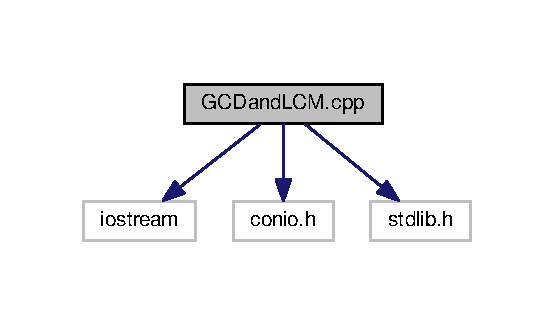
\includegraphics[width=266pt]{GCDandLCM_8cpp__incl}
\end{center}
\end{figure}
\subsection*{Functions}
\begin{DoxyCompactItemize}
\item 
int \hyperlink{GCDandLCM_8cpp_a6643c204235347beac39d3a1a3b95a1d}{gcd} (int x, int y)
\item 
int \hyperlink{GCDandLCM_8cpp_a98322a6b70154a529f32340d34e43c65}{lcm} (int x, int y)
\item 
int \hyperlink{GCDandLCM_8cpp_a3c04138a5bfe5d72780bb7e82a18e627}{main} (int argc, char $\ast$$\ast$argv)
\end{DoxyCompactItemize}


\subsection{Function Documentation}
\index{G\+C\+Dand\+L\+C\+M.\+cpp@{G\+C\+Dand\+L\+C\+M.\+cpp}!gcd@{gcd}}
\index{gcd@{gcd}!G\+C\+Dand\+L\+C\+M.\+cpp@{G\+C\+Dand\+L\+C\+M.\+cpp}}
\subsubsection[{\texorpdfstring{gcd(int x, int y)}{gcd(int x, int y)}}]{\setlength{\rightskip}{0pt plus 5cm}int gcd (
\begin{DoxyParamCaption}
\item[{int}]{x, }
\item[{int}]{y}
\end{DoxyParamCaption}
)}\hypertarget{GCDandLCM_8cpp_a6643c204235347beac39d3a1a3b95a1d}{}\label{GCDandLCM_8cpp_a6643c204235347beac39d3a1a3b95a1d}

\begin{DoxyCode}
8 \{
9     \textcolor{keywordtype}{int} r = 0, a, b;
10     a = (x > y) ? x : y; \textcolor{comment}{// a is greater number}
11     b = (x < y) ? x : y; \textcolor{comment}{// b is smaller number}
12  
13     r = b;
14     \textcolor{keywordflow}{while} (a % b != 0)
15     \{
16         r = a % b;
17         a = b;
18         b = r;
19     \}
20     \textcolor{keywordflow}{return} r;
21 \}
\end{DoxyCode}
\index{G\+C\+Dand\+L\+C\+M.\+cpp@{G\+C\+Dand\+L\+C\+M.\+cpp}!lcm@{lcm}}
\index{lcm@{lcm}!G\+C\+Dand\+L\+C\+M.\+cpp@{G\+C\+Dand\+L\+C\+M.\+cpp}}
\subsubsection[{\texorpdfstring{lcm(int x, int y)}{lcm(int x, int y)}}]{\setlength{\rightskip}{0pt plus 5cm}int lcm (
\begin{DoxyParamCaption}
\item[{int}]{x, }
\item[{int}]{y}
\end{DoxyParamCaption}
)}\hypertarget{GCDandLCM_8cpp_a98322a6b70154a529f32340d34e43c65}{}\label{GCDandLCM_8cpp_a98322a6b70154a529f32340d34e43c65}

\begin{DoxyCode}
24 \{
25     \textcolor{keywordtype}{int} a;
26     a = (x > y) ? x : y; \textcolor{comment}{// a is greater number}
27     \textcolor{keywordflow}{while} (\textcolor{keyword}{true})
28     \{
29         \textcolor{keywordflow}{if} (a % x == 0 && a % y == 0)
30             \textcolor{keywordflow}{return} a;
31         ++a;
32     \}
33 \}
\end{DoxyCode}
\index{G\+C\+Dand\+L\+C\+M.\+cpp@{G\+C\+Dand\+L\+C\+M.\+cpp}!main@{main}}
\index{main@{main}!G\+C\+Dand\+L\+C\+M.\+cpp@{G\+C\+Dand\+L\+C\+M.\+cpp}}
\subsubsection[{\texorpdfstring{main(int argc, char $\ast$$\ast$argv)}{main(int argc, char **argv)}}]{\setlength{\rightskip}{0pt plus 5cm}int main (
\begin{DoxyParamCaption}
\item[{int}]{argc, }
\item[{char $\ast$$\ast$}]{argv}
\end{DoxyParamCaption}
)}\hypertarget{GCDandLCM_8cpp_a3c04138a5bfe5d72780bb7e82a18e627}{}\label{GCDandLCM_8cpp_a3c04138a5bfe5d72780bb7e82a18e627}

\begin{DoxyCode}
36 \{
37     cout << \textcolor{stringliteral}{"Enter the two numbers: "};
38     \textcolor{keywordtype}{int} x, y;
39     cin >> x >> y;
40     cout << \textcolor{stringliteral}{"The GCD of two numbers is: "} << \hyperlink{GCDandLCM_8cpp_a6643c204235347beac39d3a1a3b95a1d}{gcd}(x, y) << endl;
41     ;
42     cout << \textcolor{stringliteral}{"The LCM of two numbers is: "} << \hyperlink{GCDandLCM_8cpp_a98322a6b70154a529f32340d34e43c65}{lcm}(x, y) << endl;
43     ;
44     \textcolor{keywordflow}{return} 0;
45 \}\end{DoxyCode}


Here is the call graph for this function\+:
\nopagebreak
\begin{figure}[H]
\begin{center}
\leavevmode
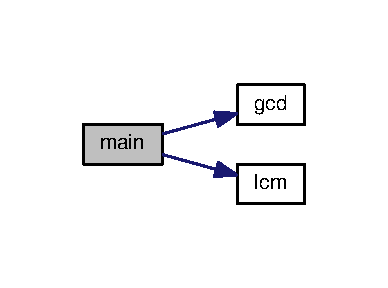
\includegraphics[width=186pt]{GCDandLCM_8cpp_a3c04138a5bfe5d72780bb7e82a18e627_cgraph}
\end{center}
\end{figure}



%--- End generated contents ---

% Index
\backmatter
\newpage
\phantomsection
\clearemptydoublepage
\addcontentsline{toc}{chapter}{Index}
\printindex

\end{document}
